\documentclass[11pt,a4paper]{article}
\usepackage[margin=2.3cm]{geometry}
\usepackage{amsmath,amssymb}
\usepackage{graphicx}
\usepackage{booktabs}
\usepackage{float}
\usepackage{caption}
\usepackage{siunitx}
\usepackage[hidelinks]{hyperref}
\captionsetup{font=small,labelfont=bf}
\renewcommand{\arraystretch}{1.1}
\graphicspath{{figures/}}
\sisetup{separate-uncertainty=true}

\title{\textbf{Blackbody Radiation}\\[2pt]\large Laboratory Report}
\author{Parth\\SR No.\ 26788}
\date{Date of experiment: 26 October 2026}

\begin{document}
\maketitle

\section{Aim}
To study the radiation emitted by the incandescent tungsten filament of a bulb, treated as a blackbody, by
\begin{enumerate}
  \item determining the filament temperature at several bulb voltages from its electrical resistance,
  \item measuring the intensity of the emitted light as a function of angular position with a prism spectrophotometer, converting angle to wavelength and finding the wavelength $\lambda_{\max}$ of maximum intensity,
  \item verifying Stefan's law ($I\propto T^{4}$), and
  \item verifying Wien's displacement law ($\lambda_{\max}T=\text{const.}$) and estimating Wien's constant.
\end{enumerate}

\section{Theory}

\subsection{Blackbody radiation}
A blackbody is an ideal body that absorbs all radiation falling on it. In thermal equilibrium it must also emit as efficiently as it absorbs, and the spectrum it emits depends \emph{only} on its temperature and not on its material or shape. A small hole in a closed cavity whose walls are held at temperature $T$ is the standard realisation. Classical physics failed to explain the measured spectrum: the Rayleigh--Jeans law, derived from equipartition of energy among the electromagnetic modes of the cavity, gives a spectral radiance
\begin{equation}
  B_\lambda^{\rm RJ}(T)=\frac{2ck_BT}{\lambda^{4}},
\end{equation}
which agrees with experiment at long wavelengths but diverges as $\lambda\to0$ (the ``ultraviolet catastrophe'') and predicts an infinite total power. In 1900 Max Planck removed the divergence by postulating that the cavity oscillators can exchange energy with the radiation field only in discrete units $E=h\nu$, which marks the beginning of quantum mechanics.

\subsection{Planck's law}
With the energy of an oscillator of frequency $\nu$ restricted to $E_n=nh\nu$, its mean energy at temperature $T$ is $\bar E=h\nu/(e^{h\nu/k_BT}-1)$ instead of the classical $k_BT$. The spectral radiance (power per unit area, per unit solid angle, per unit wavelength) is then
\begin{equation}
  B_\lambda(T)=\frac{2hc^{2}}{\lambda^{5}}\,\frac{1}{e^{hc/\lambda k_BT}-1},
  \label{eq:planck}
\end{equation}
where $h=6.626\times10^{-34}$~J\,s, $c=2.998\times10^{8}$~m\,s$^{-1}$ and $k_B=1.381\times10^{-23}$~J\,K$^{-1}$. For $\lambda\gg hc/k_BT$ Eq.~\eqref{eq:planck} reduces to the Rayleigh--Jeans law, and for $\lambda\ll hc/k_BT$ to Wien's approximation $B_\lambda\approx(2hc^2/\lambda^5)\,e^{-hc/\lambda k_BT}$. Figure~\ref{fig:theory} shows the black-body spectrum for several temperatures: the curve rises steeply on the short-wavelength side, passes through a single maximum and falls slowly on the long-wavelength side; as $T$ increases the total area grows rapidly and the peak moves to shorter wavelengths.

\begin{figure}[H]
\centering
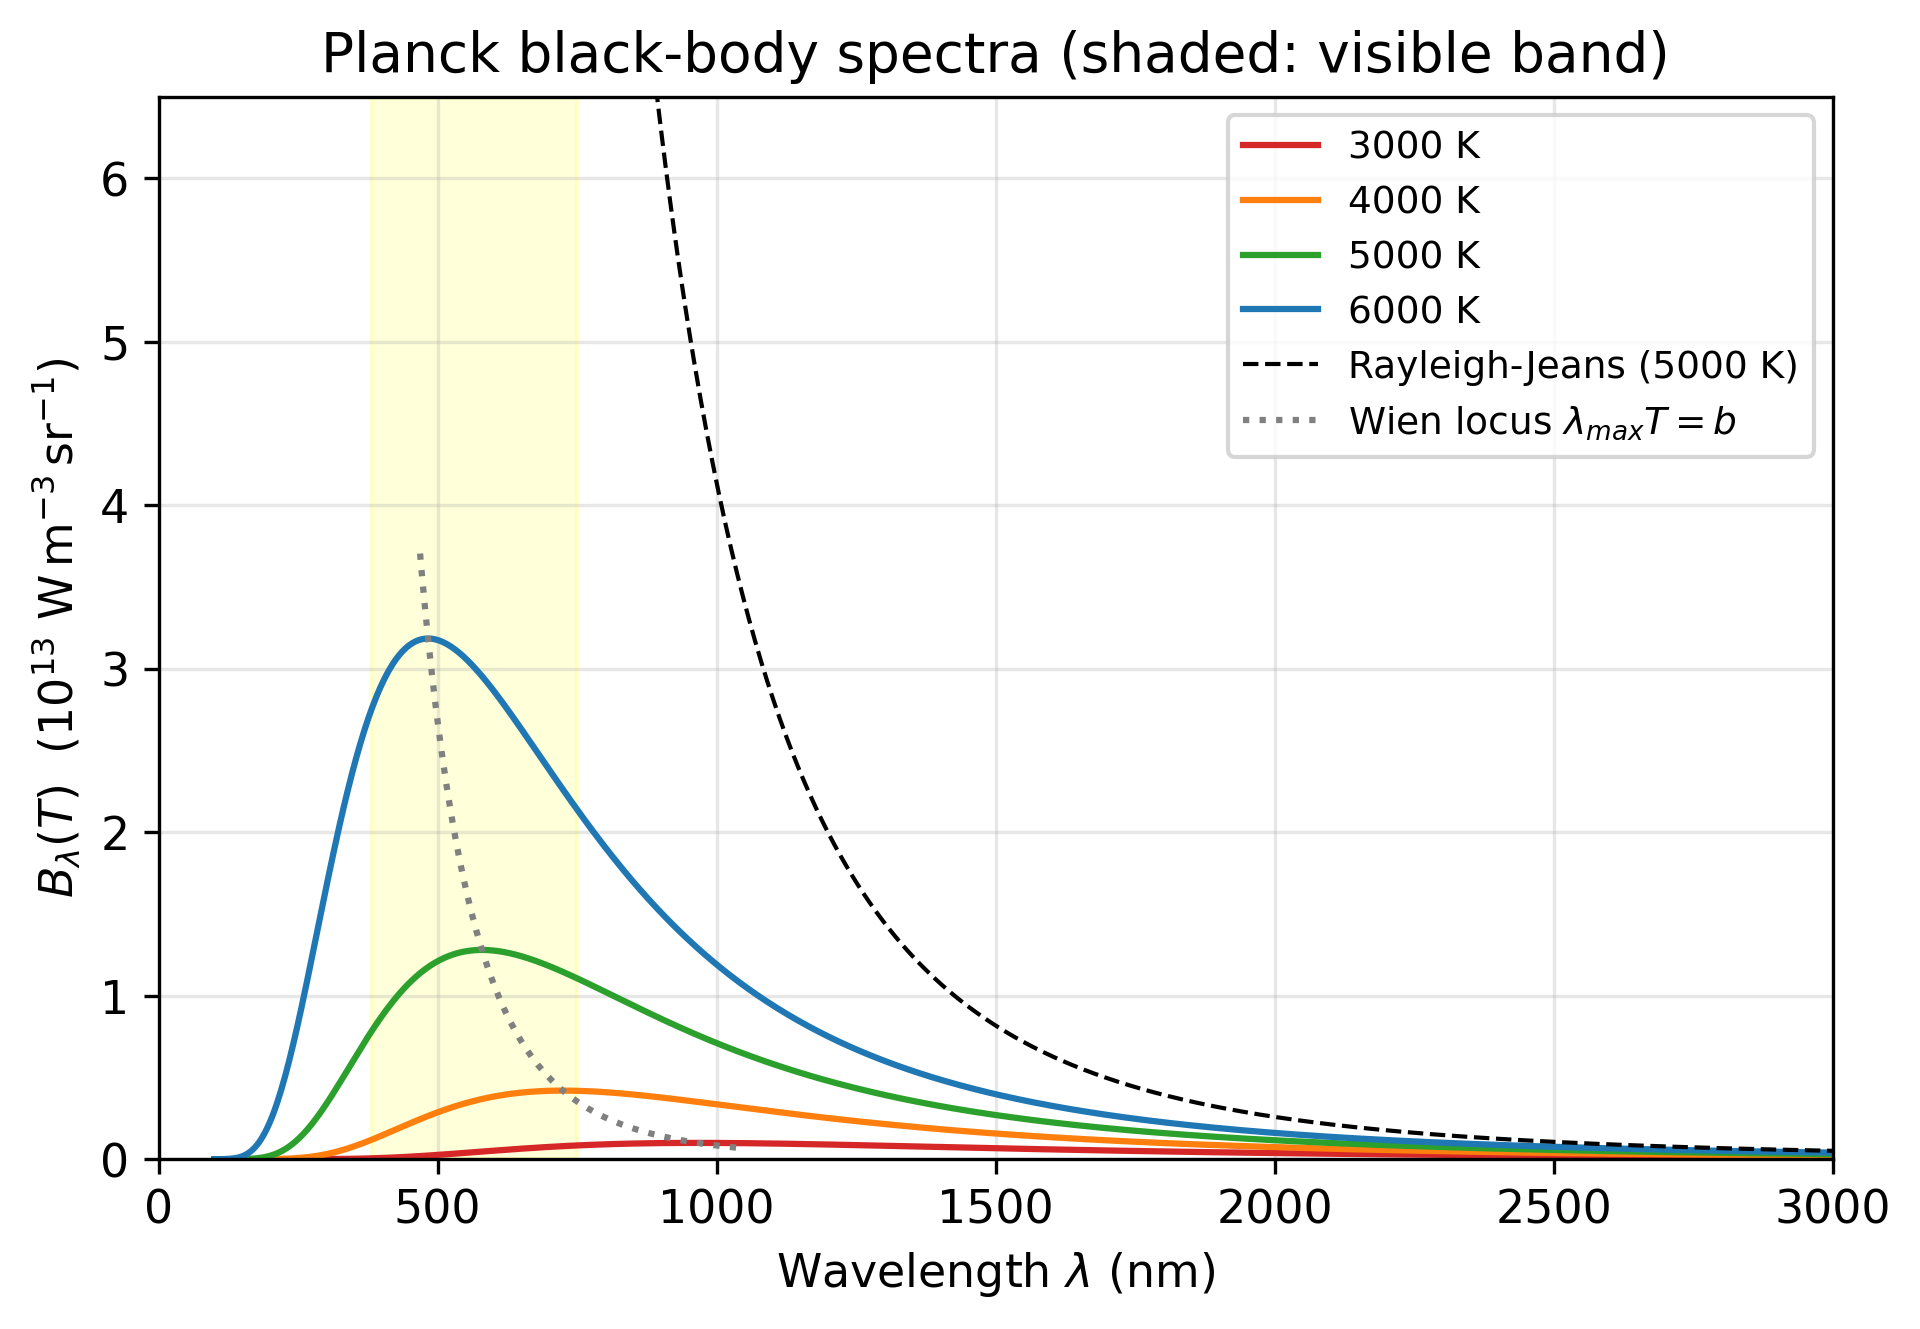
\includegraphics[width=0.78\textwidth]{fig2_blackbody_spectrum_theory.png}
\caption{Black-body spectra from Planck's law for four temperatures, the classical Rayleigh--Jeans curve (5000~K) and the locus of the maxima (Wien's law).}
\label{fig:theory}
\end{figure}

\subsection{Stefan's law}
Integrating Eq.~\eqref{eq:planck} over all wavelengths and over the hemisphere gives the total power radiated per unit area of a blackbody,
\begin{equation}
  M=\int_0^\infty\!\!\pi B_\lambda\,\mathrm{d}\lambda=\sigma T^{4},\qquad
  \sigma=\frac{2\pi^{5}k_B^{4}}{15\,c^{2}h^{3}}=5.67\times10^{-8}\ \mathrm{W\,m^{-2}\,K^{-4}}.
\end{equation}
Hence the total detected intensity should obey $I_{\rm tot}=kT^{4}$, i.e.
\begin{equation}
  \ln I_{\rm tot}=4\ln T+\ln k ,
  \label{eq:stefan}
\end{equation}
so a plot of $\ln I_{\rm tot}$ against $\ln T$ is a straight line of slope $\approx4$. A real body with emissivity $\varepsilon<1$ (tungsten has $\varepsilon\approx0.3$--$0.4$ in this range) radiates $\varepsilon\sigma T^4$; if $\varepsilon$ varies only slowly with $T$ the slope is still close to 4.

\subsection{Wien's displacement law}
Setting $\mathrm{d}B_\lambda/\mathrm{d}\lambda=0$ and writing $x=hc/\lambda k_BT$ gives the transcendental equation $(x-5)e^{x}+5=0$, whose root is $x=4.965$. The wavelength of maximum emission therefore satisfies
\begin{equation}
  \lambda_{\max}T=b,\qquad b=\frac{hc}{4.965\,k_B}=2.898\times10^{-3}\ \mathrm{m\,K}.
  \label{eq:wien}
\end{equation}
A graph of $\lambda_{\max}$ against $1/T$ is a straight line through the origin with slope $b$.

\subsection{The filament as a blackbody and its temperature}
The filament of an incandescent bulb is a hot, opaque, tightly coiled tungsten wire; the coil traps most of its own radiation (cavity-like) so its spectrum is close to that of a (grey) blackbody of the filament temperature. The temperature follows from the temperature dependence of the resistance of tungsten,
\begin{equation}
  R=R_0\,[1+\alpha_0\,(T-T_0)]\quad\Longrightarrow\quad T=T_0+\frac{1}{\alpha_0}\left(\frac{R}{R_0}-1\right),
  \label{eq:temp}
\end{equation}
where $R_0$ is the resistance at room temperature $T_0$ and $\alpha_0=4.5\times10^{-3}$~K$^{-1}$. (The handout prints a minus sign in the bracket; this is a typographical error, since the resistance of a metal increases with temperature.) $R_0$ is found from the slope of the $V$--$I$ graph at a voltage so small that the filament does not heat up, and $R=V/I$ at the working voltage.

\subsection{Wavelength from the prism deviation angle}
The $60^\circ$ prism disperses the light, and the Rotary Motion Sensor records the angle $\theta$ of the emergent ray measured from the undeviated beam ($\theta_0$). With the beam incident at $60^\circ$ on the first face of a prism of apex angle $60^\circ$, the refractive index is
\begin{equation}
  n=\sqrt{\left(\frac{2}{\sqrt3}\sin\theta+\frac12\right)^{2}+\frac34},
  \label{eq:n}
\end{equation}
and the dispersion of the glass is described by Cauchy's relation
\begin{equation}
  n=\frac{A}{\lambda^{2}}+B,\qquad A=13\,900\ \mathrm{nm^{2}},\quad B=1.689 ,
  \label{eq:cauchy}
\end{equation}
so that
\begin{equation}
  \lambda=\sqrt{\frac{A}{n-B}}\ \ (\text{nm}).
  \label{eq:lambda}
\end{equation}
Equation~\eqref{eq:lambda} is defined only for $n>B$, i.e.\ for $\theta>55.37^\circ$; wavelengths longer than about 1.3~$\mu$m are squeezed into less than $1^\circ$ of arm angle.

\section{Calculations and Results}

\subsection{Resistance of the filament at room temperature}
With small applied voltages (0.01--0.10~V, maximum dissipation 2.7~mW) the filament stays at room temperature and obeys Ohm's law. Figure~\ref{fig:vi} shows the $V$--$I$ graph. A least-squares fit $V=R_0I+c$ gives
\begin{equation}
  R_0=3.62\pm0.09\ \Omega,\qquad c=0.001\pm0.002\ \text{V}\ (\text{consistent with zero}),\qquad r=0.998 .
\end{equation}
A fit forced through the origin gives $R_0=3.68\pm0.04~\Omega$, and the value noted in the laboratory notebook is $3.66~\Omega$; all three agree within the uncertainty. The fitted slope $R_0=3.62~\Omega$ is used below. The room temperature was not recorded and is taken as $T_0=300\pm3$~K.

\begin{figure}[H]
\centering
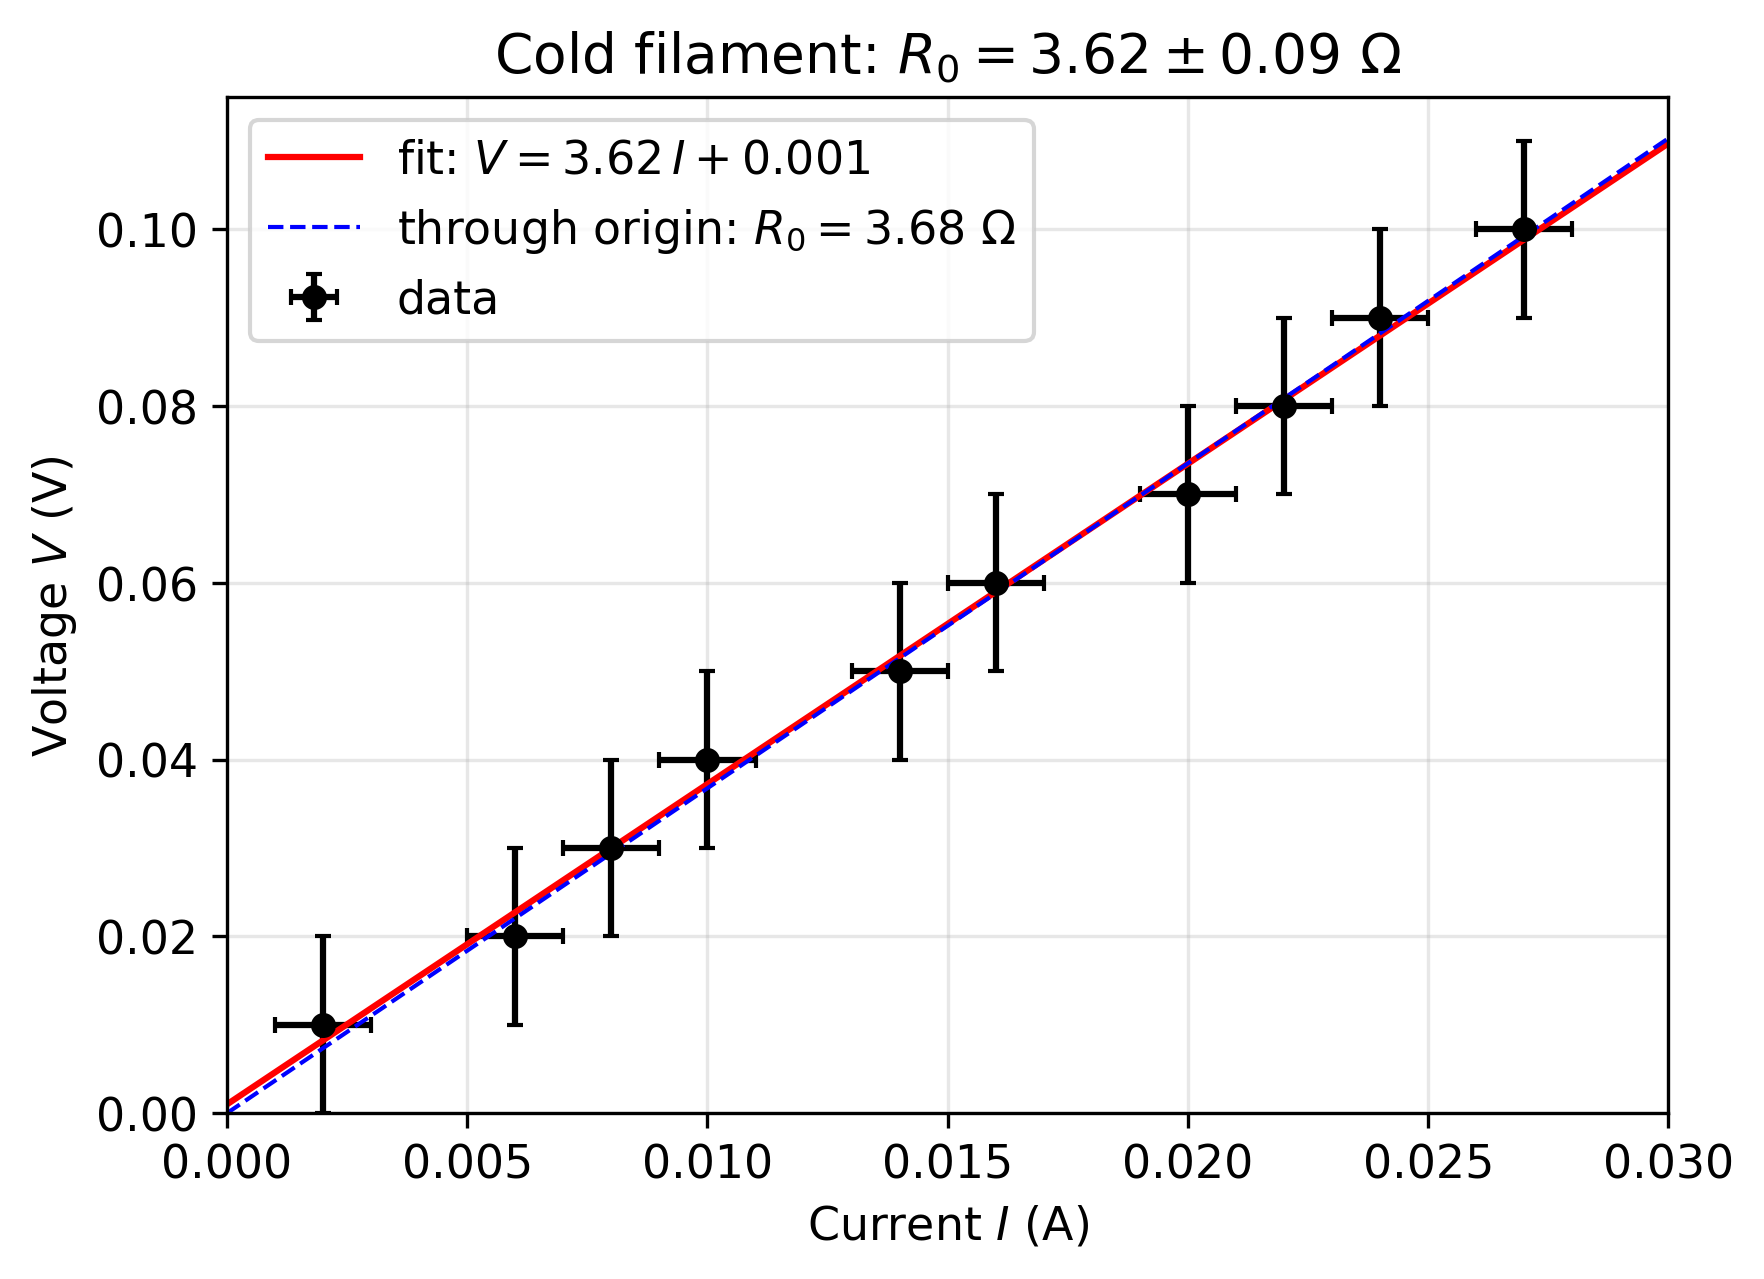
\includegraphics[width=0.62\textwidth]{fig1_resistance_room_temperature.png}
\caption{Voltage against current for the cold filament; the slope gives $R_0$.}
\label{fig:vi}
\end{figure}

\subsection{Temperature of the filament}
At each bulb voltage the current was noted and $R=V/I$ and $T$ were obtained from Eq.~\eqref{eq:temp}. \emph{Worked example, 6.00~V:}
\begin{align*}
R&=\frac{6.00}{0.256}=23.44\ \Omega,\qquad \frac{R}{R_0}=\frac{23.44}{3.62}=6.47,\\
T&=300+\frac{6.47-1}{4.5\times10^{-3}}=300+1215\approx1515\ \text{K}.
\end{align*}
\begin{table}[H]
\centering
\begin{tabular}{ccccccc}
\toprule
Run & $V$ (V) & $I$ (A) & $P=VI$ (W) & $R$ ($\Omega$) & $T$ (K) & $T$ ($^\circ$C)\\
\midrule
5  & 6.0 & 0.256 & 1.54 & $23.44\pm0.10$ & $1515\pm36$ & 1242\\
6  & 7.0 & 0.280 & 1.96 & $25.00\pm0.10$ & $1611\pm39$ & 1337\\
12 & 7.5 & 0.290 & 2.18 & $25.86\pm0.10$ & $1663\pm40$ & 1390\\
9  & 8.0 & 0.300 & 2.40 & $26.67\pm0.09$ & $1713\pm41$ & 1440\\
\bottomrule
\end{tabular}
\caption{Filament resistance and temperature at the four bulb voltages used. (Readings at 6.5~V and 9~V were struck out in the notebook and are not used.)}
\label{tab:T}
\end{table}

\subsection{Intensity as a function of angular position}
The angular position was zeroed with the undeviated white beam centred on the aperture slit ($\theta_0=0$), so the emergent angle is $\theta=|\text{reading}|$. The sensor values are taken directly as the arm angle in degrees (the calibration run, which records the angle channel against the calibrated angle channel, gives a straight line of slope $1.000$ and intercept $0$, so no rescaling was needed). The recorded intensity is a percentage of the full scale of the light sensor, and each run has its own constant offset ($-7$\% to $+1$\%) because the sensor zero was re-set between runs.

Figure~\ref{fig:angle} shows the intensity against angle for the four voltages. Away from the feature the signal is flat or drifts slowly (stray and room light). Between $\theta\approx56^\circ$ and $63^\circ$ there is a single smooth peak that grows with the bulb voltage and moves slightly towards larger angles. For the analysis a straight-line baseline was fitted to line-free windows on either side ($53^\circ$--$55.8^\circ$ and $64.5^\circ$--$68^\circ$; rms residual 0.05--0.07\,\%) and subtracted (Fig.~\ref{fig:angle}b).

\begin{figure}[H]
\centering
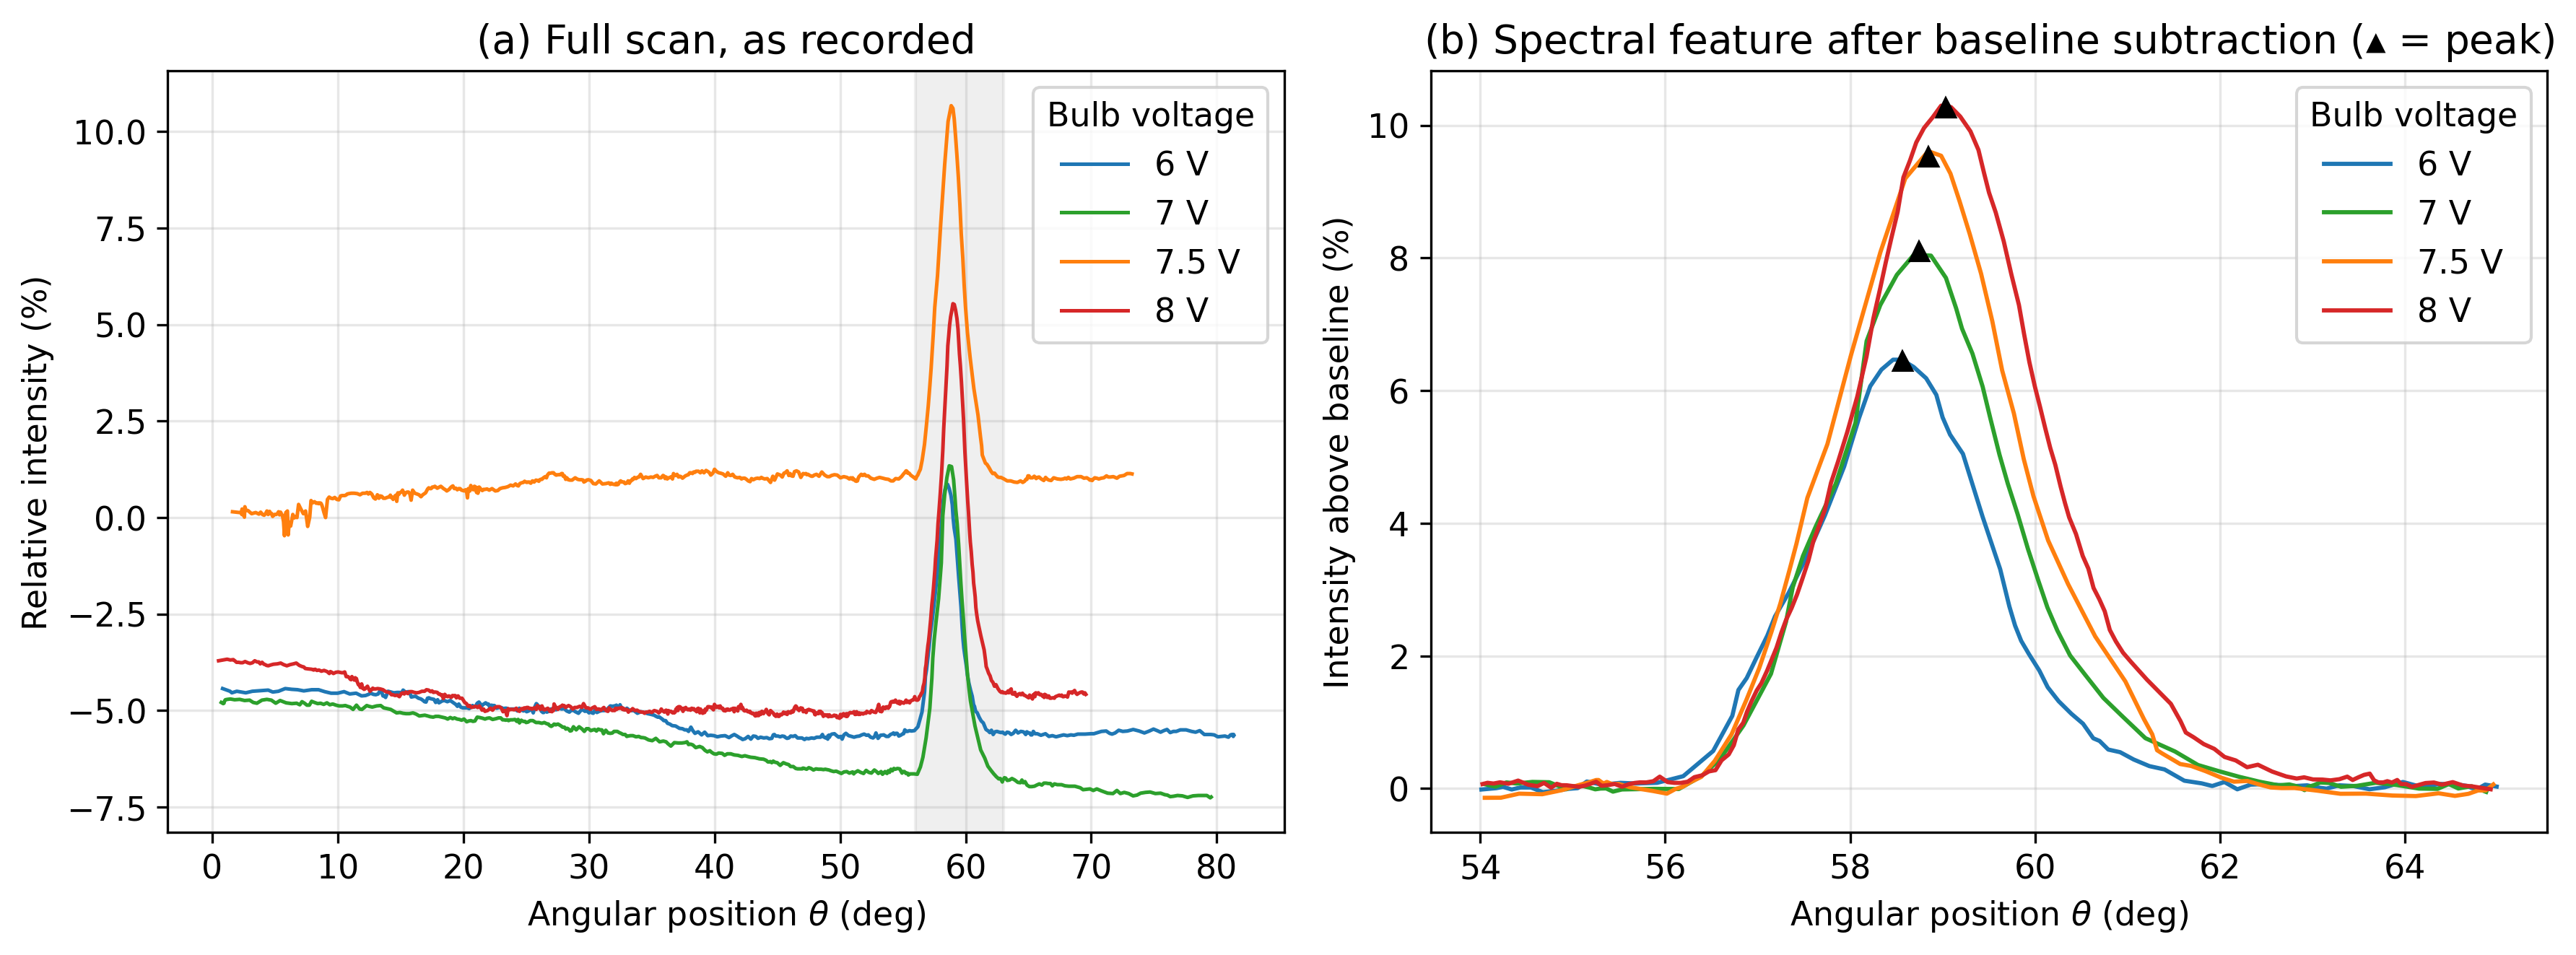
\includegraphics[width=\textwidth]{fig3_intensity_vs_angle.png}
\caption{Relative intensity against angular position for bulb voltages of 6, 7, 7.5 and 8~V. (a)~Full scans as recorded (shaded band: region of the spectral feature). (b)~The feature after baseline subtraction; triangles mark the fitted peak positions.}
\label{fig:angle}
\end{figure}

\subsection{Intensity as a function of wavelength and $\lambda_{\max}$}
Each angle was converted to a wavelength with Eqs.~\eqref{eq:n}--\eqref{eq:lambda}. \emph{Worked example, 6.0~V:} the peak is at $\theta=58.57^\circ$ (vertex of a parabola fitted to the points within $\pm0.7^\circ$ of the maximum), so
\begin{align*}
n&=\sqrt{\left(\tfrac{2}{\sqrt3}\sin58.57^\circ+\tfrac12\right)^{2}+\tfrac34}
=\sqrt{(0.9853+0.5)^2+0.75}=1.7193,\\
\lambda_{\max}&=\sqrt{\frac{13\,900}{1.7193-1.689}}=\sqrt{\frac{13\,900}{0.0303}}\approx677\ \text{nm}.
\end{align*}
The uncertainty $\pm0.10^\circ$ in $\theta$ (fit error combined with the $0.1^\circ$ reading uncertainty) corresponds to $\pm10$~nm. Figure~\ref{fig:lambda} shows the baseline-subtracted intensity against wavelength, and Table~\ref{tab:spec} lists the results.

\begin{figure}[H]
\centering
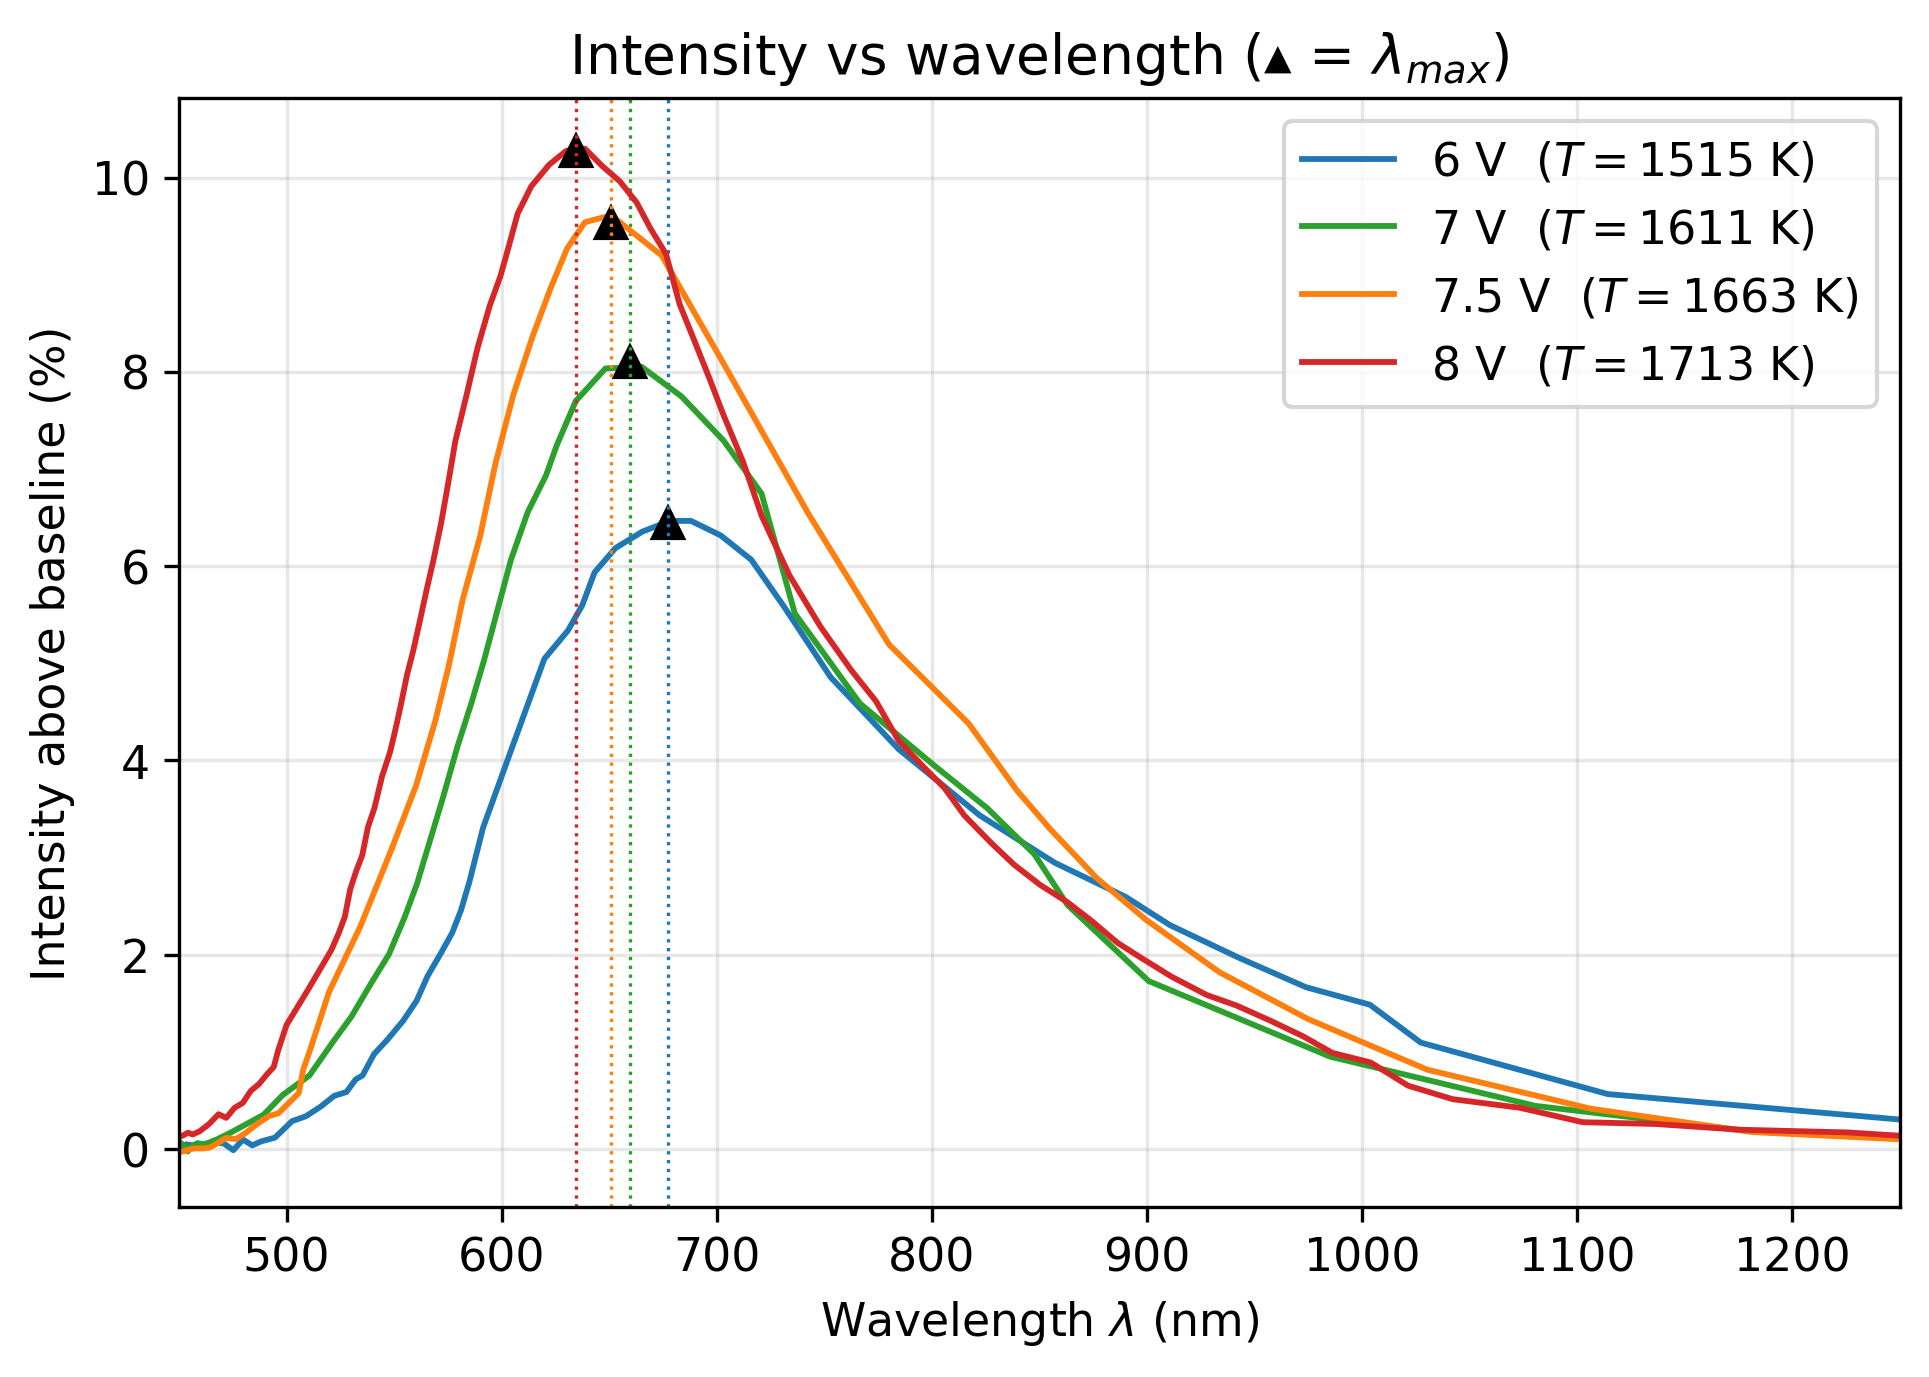
\includegraphics[width=0.78\textwidth]{fig4_intensity_vs_wavelength.png}
\caption{Intensity against wavelength for the four bulb temperatures. The triangles and dotted lines mark $\lambda_{\max}$.}
\label{fig:lambda}
\end{figure}

\begin{table}[H]
\centering\small
\setlength{\tabcolsep}{4pt}
\begin{tabular}{cccccccc}
\toprule
$V$ (V) & $T$ (K) & $\theta_{\max}$ ($^\circ$) & $n$ & $\lambda_{\max}$ (nm) & $I_{\max}$ (\%) & $I_{\rm tot}$ (\%$\cdot^\circ$) & $\lambda_{\max}^{\rm Wien}$ (nm)\\
\midrule
6.0 & 1515 & $58.57\pm0.10$ & 1.7193 & $677\pm10$ & 6.45 & $15.4\pm0.4$ & 1913\\
7.0 & 1611 & $58.75\pm0.10$ & 1.7209 & $660\pm9$  & 8.10 & $19.3\pm0.4$ & 1799\\
7.5 & 1663 & $58.85\pm0.10$ & 1.7218 & $651\pm9$  & 9.53 & $23.7\pm0.6$ & 1742\\
8.0 & 1713 & $59.04\pm0.10$ & 1.7235 & $634\pm8$  & 10.27 & $26.1\pm0.5$ & 1692\\
\bottomrule
\end{tabular}
\caption{Peak position, refractive index, $\lambda_{\max}$, peak height above baseline, integrated intensity $I_{\rm tot}=\int I\,\mathrm{d}\theta$ over $56^\circ$--$63^\circ$, and, for comparison, the value $b/T$ expected from Wien's law with $b=2.898\times10^{-3}$~m\,K.}
\label{tab:spec}
\end{table}

As the filament gets hotter, the peak grows and shifts to \emph{shorter} wavelength (from 677 to 634~nm for a rise of about 200~K), as the blackbody picture predicts. The full width at half maximum covers roughly 560--860~nm in every run. However, the measured peaks (630--680~nm) lie far below the wavelengths $b/T\approx1.7$--$1.9~\mu$m at which a blackbody of this temperature emits most strongly (last column of Table~\ref{tab:spec}); this is discussed in Sec.~\ref{sec:conc}.

\subsection{Verification of Stefan's law}
The total (baseline-subtracted) intensity $I_{\rm tot}$ was obtained by numerically integrating each spectrum over the whole feature, $56^\circ\le\theta\le63^\circ$ (the detector collects the energy per unit angle through a slit of fixed angular width, so the integral over $\theta$ is proportional to the total detected power). Figure~\ref{fig:stefan}(a) is the graph of $\ln I_{\rm tot}$ against $\ln T$ suggested by Eq.~\eqref{eq:stefan}, and (b) shows $I_{\rm tot}$ against $T^{4}$. The least-squares line gives
\begin{equation}
  \text{slope}=4.43\pm0.34\quad(r=0.994),
\end{equation}
which agrees with the expected value of 4 within about $1.3$ standard errors. Using the peak height $I_{\max}$ instead of the integral gives $3.90\pm0.24$ ($r=0.996$), also consistent with 4; the mean of the two estimates is $\approx4.2$. As a cross-check, the electrical power $P=VI$ supplied to the bulb varies as $T^{3.64\pm0.13}$; it is somewhat below 4 because part of the input power leaves by conduction through the lead wires and gas and because the emissivity of tungsten increases with temperature.

\begin{figure}[H]
\centering
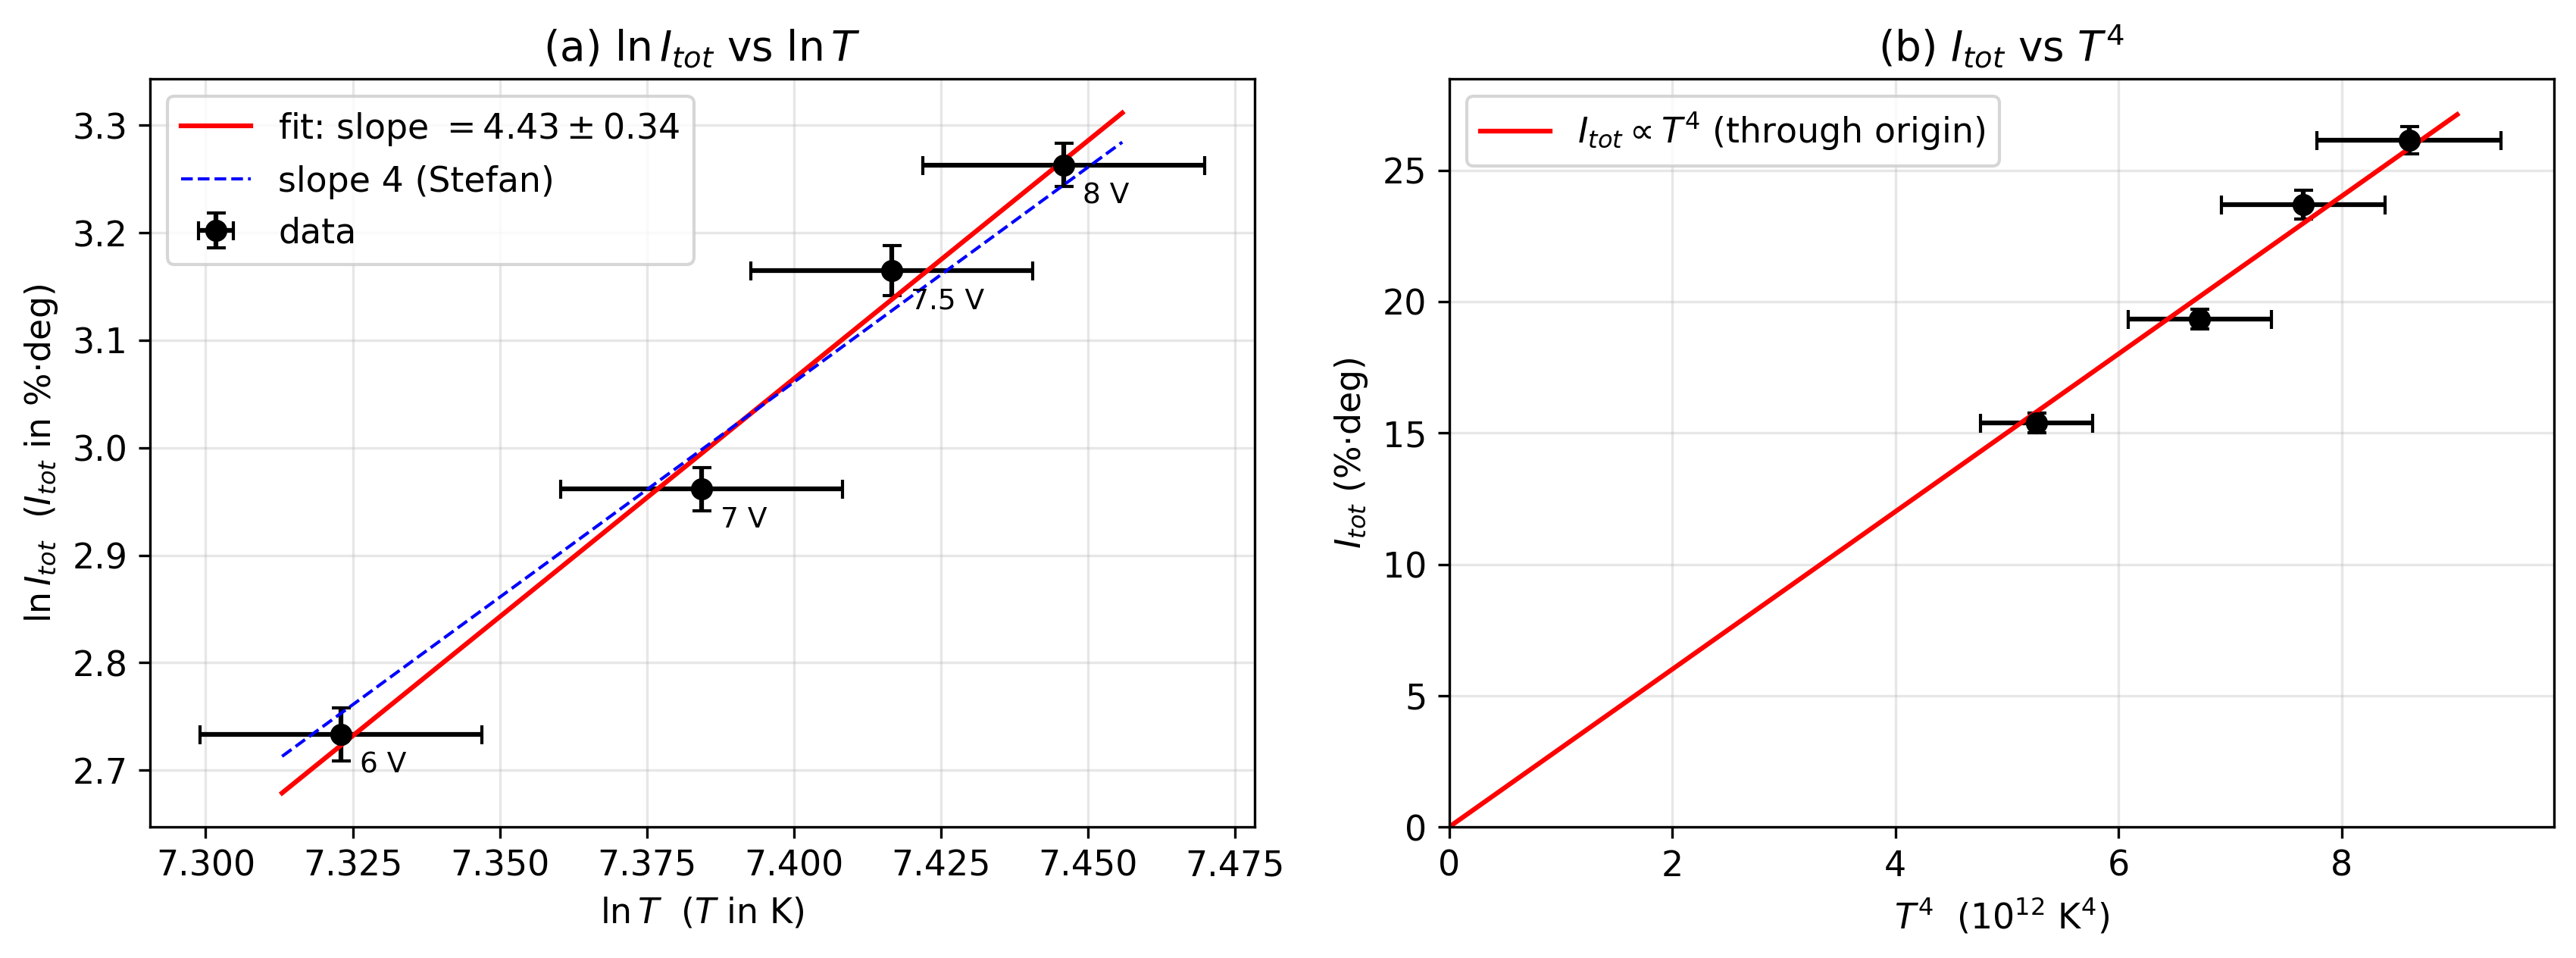
\includegraphics[width=\textwidth]{fig5_stefan_law.png}
\caption{Verification of Stefan's law. (a)~$\ln I_{\rm tot}$ against $\ln T$ with the fitted line and, for comparison, a line of slope exactly 4. (b)~$I_{\rm tot}$ against $T^{4}$ with a straight line through the origin.}
\label{fig:stefan}
\end{figure}

\subsection{Verification of Wien's displacement law}
Figure~\ref{fig:wien}(a) shows $\lambda_{\max}$ against $1/T$ and (b) the product $\lambda_{\max}T$ against $T$. Fitting $\lambda_{\max}=b/T$ (line through the origin) gives
\begin{equation}
  b=(1.06\pm0.01)\times10^{6}\ \text{nm\,K}=(1.06\pm0.01)\times10^{-3}\ \text{m\,K},
\end{equation}
where the quoted error is the statistical error of the fit only. The product $\lambda_{\max}T$ is nearly constant over the range studied: $1.03$, $1.06$, $1.08$, $1.09$ $(\times10^{-3}\ \text{m\,K})$ for 6, 7, 7.5 and 8~V, mean $(1.06\pm0.03)\times10^{-3}$~m\,K (scatter 2.6\,\%), i.e.\ $\lambda_{\max}$ varies approximately as $1/T$ in the sense of Wien's law. A free straight-line fit $\lambda_{\max}=a+s/T$ gives $s=(5.4\pm0.7)\times10^{5}$~nm\,K and $a=325\pm44$~nm ($r=0.983$), and a log--log fit gives $\lambda_{\max}\propto T^{-0.51\pm0.06}$ (Wien's law: $-1$). These two fits are poorly constrained because $T$ spans only 13\,\% (1515--1713~K) and the uncertainty in $T$ ($\pm2.4\,\%$) is comparable to the whole change in $\lambda_{\max}$ ($-6\,\%$), so they should be regarded as indicative only.

The measured coefficient is $b_{\rm exp}=1.06\times10^{-3}$~m\,K, which is only $37\,\%$ of the accepted value $2.898\times10^{-3}$~m\,K (a deviation of $-63\,\%$). Wien's law is therefore confirmed in its qualitative form (the peak moves to shorter wavelength as $T$ rises and $\lambda_{\max}T$ is approximately constant), but not quantitatively.

\begin{figure}[H]
\centering
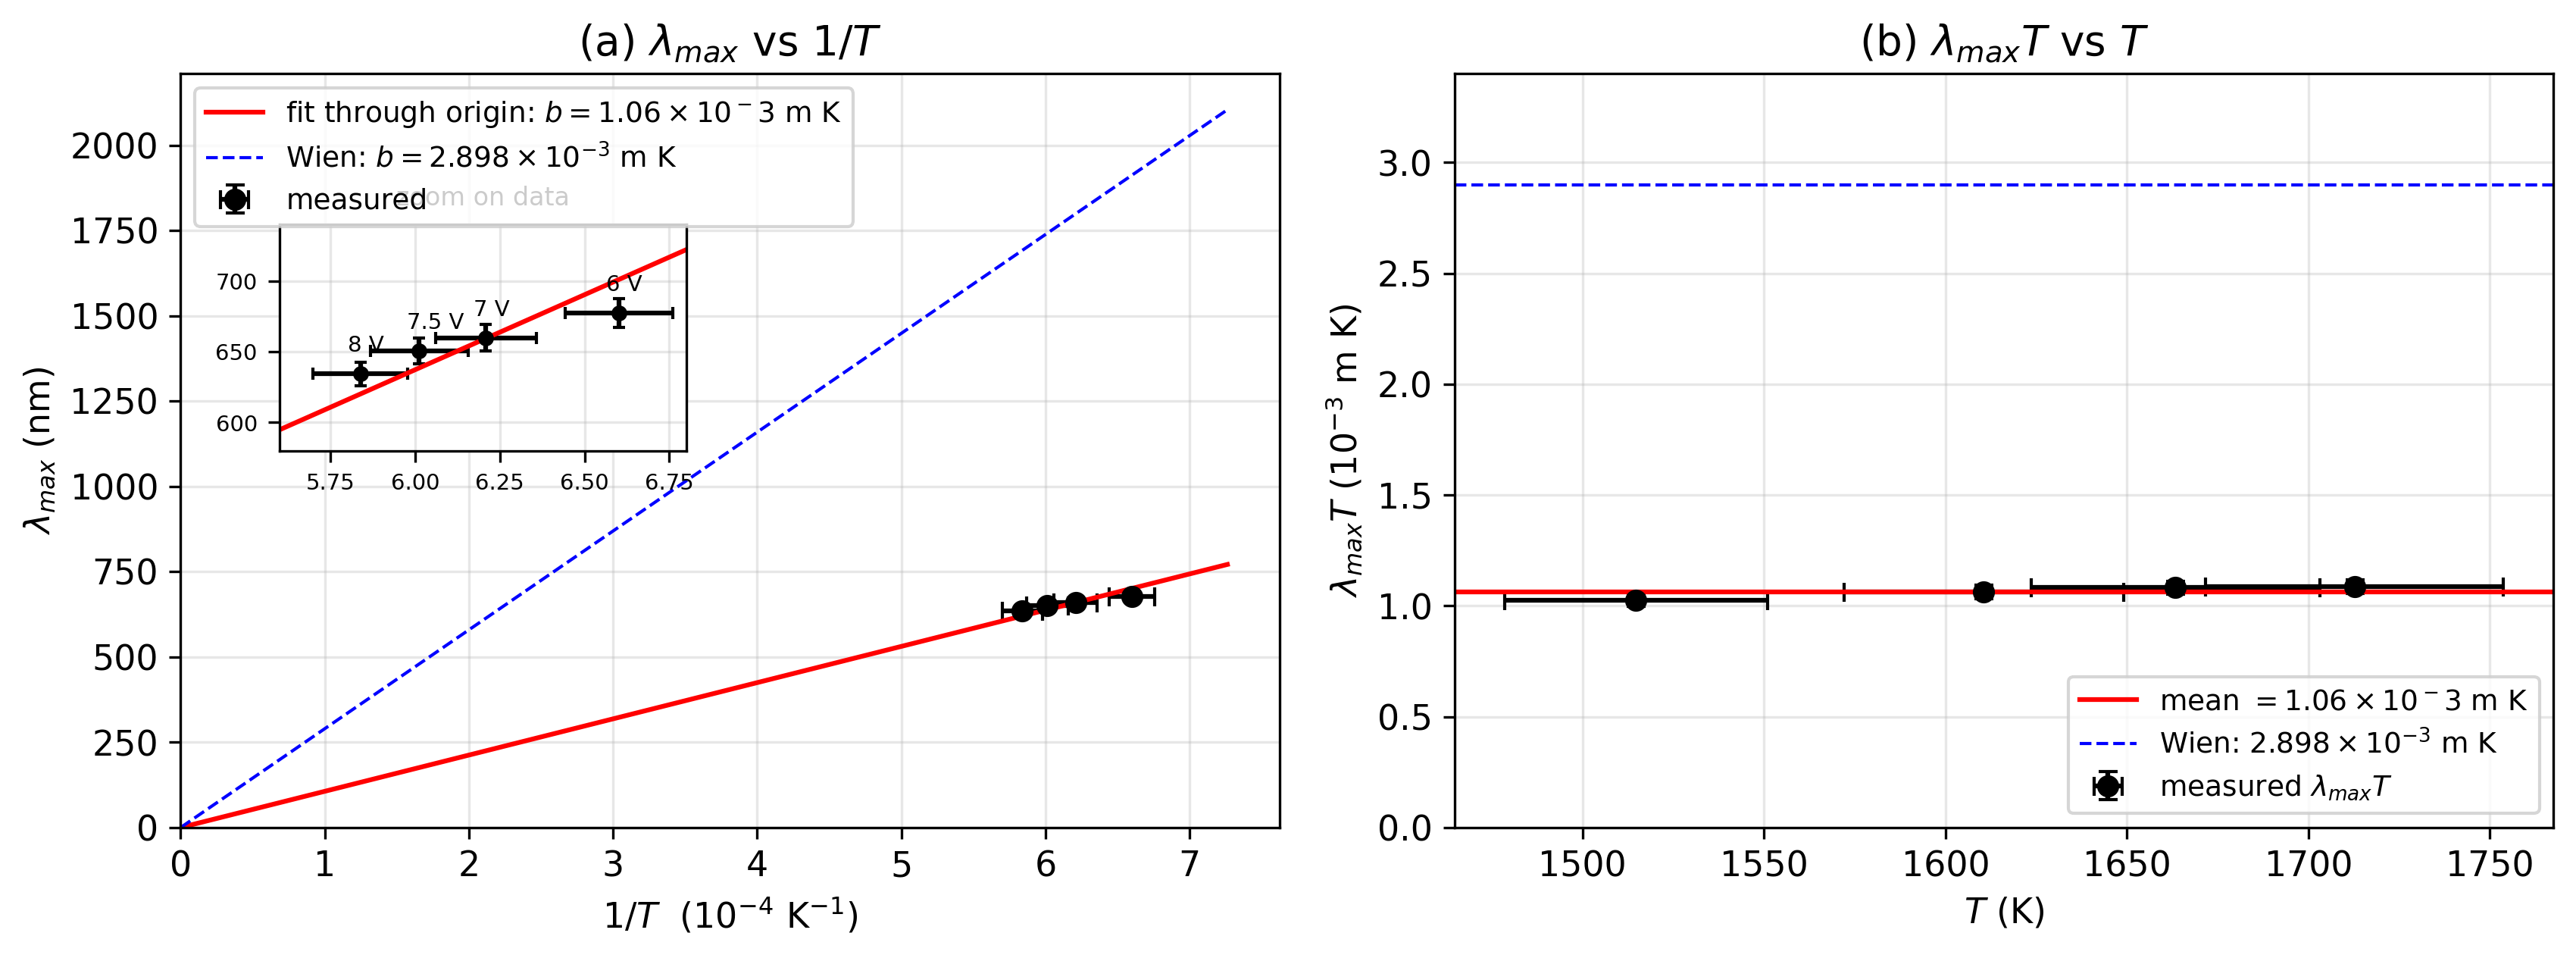
\includegraphics[width=\textwidth]{fig6_wien_law.png}
\caption{Verification of Wien's law. (a)~$\lambda_{\max}$ against $1/T$ with the fit through the origin and the line for the accepted $b=2.898\times10^{-3}$~m\,K; the inset magnifies the data. (b)~$\lambda_{\max}T$ against $T$.}
\label{fig:wien}
\end{figure}

\section{Error Analysis}
\begin{itemize}
  \item \textbf{Resistance and temperature.} $V$ and $I$ were read to $\pm0.01$~V and $\pm0.001$~A, giving $\Delta R\approx0.1~\Omega$ at the working points. The error in $R_0$ ($\pm0.09~\Omega$, 2.5\,\%, from the fit) and the assumed $\Delta T_0=3$~K dominate: combining them with $\Delta R$ in quadrature in Eq.~\eqref{eq:temp} gives $\Delta T=36$--41~K ($\approx2.4\,\%$). There is also an unquantified \emph{systematic} error because Eq.~\eqref{eq:temp} treats $\alpha_0$ as constant up to $\approx1700$~K and $T_0$ was not measured. The temperatures are nevertheless consistent with tabulated tungsten resistivity at these temperatures, and since the same $R_0$, $T_0$ and $\alpha_0$ enter all runs they mostly cancel in the slope of the Stefan plot.
  \item \textbf{Angle and wavelength.} The peak position is uncertain by $\pm0.10^\circ$ (parabola-fit error and $0.1^\circ$ reading/zero uncertainty), which gives $\Delta\lambda_{\max}\approx8$--10~nm ($1.3$--$1.5\,\%$). Because $\lambda$ depends strongly on $\theta$ (about 90~nm per degree near the peak and increasing rapidly towards $55.4^\circ$), any error in the zero $\theta_0$ of the angle scale shifts all $\lambda_{\max}$ together. An error of $1^\circ$ in $\theta_0$ would change $\lambda_{\max}$ by about 90~nm.
  \item \textbf{Intensity and Stefan's law.} The rms noise of the baseline (0.05--0.07\,\%) gives $\Delta I_{\rm tot}\approx0.4$--0.6\,\%$\cdot^\circ$ (2--3\,\%). The slope of the Stefan plot is $4.43\pm0.34$ (statistical standard error of the fit, $\approx8\,\%$); with only four points this is a limited test. The comparison of intensities between runs assumes that the sensor gain was the same in all runs.
  \item \textbf{Wien's constant.} The scatter of $\lambda_{\max}T$ is 2.6\,\% and the statistical error of $b$ is only 1.3\,\%, but the systematic deviation of $b$ from the accepted value (63\,\%) is much larger than any of the random errors estimated above and therefore has a physical origin, discussed in the conclusions.
\end{itemize}

\section{Summary and Conclusions}\label{sec:conc}
\begin{table}[H]
\centering
\begin{tabular}{p{0.46\textwidth}p{0.46\textwidth}}
\toprule
Result & Value\\
\midrule
Cold resistance of filament (from $V$--$I$ graph) & $R_0=3.62\pm0.09~\Omega$\\
Filament temperature at 6, 7, 7.5, 8~V & 1515, 1611, 1663, 1713~K ($\pm$ 36--41~K)\\
Wavelength of maximum intensity & 677, 660, 651, 634~nm ($\pm$ 8--10~nm)\\
Slope of $\ln I_{\rm tot}$ vs $\ln T$ (Stefan; expected 4) & $4.43\pm0.34$ (from peak heights: $3.90\pm0.24$)\\
$\lambda_{\max}T$ (mean of four runs) & $(1.06\pm0.03)\times10^{-3}$~m\,K\\
Wien's constant $b$ (fit through origin) & $(1.06\pm0.01)\times10^{-3}$~m\,K (accepted $2.898\times10^{-3}$)\\
\bottomrule
\end{tabular}
\end{table}
\begin{itemize}
  \item The $V$--$I$ graph of the cold filament is linear ($r=0.998$) and gives $R_0=3.62\pm0.09~\Omega$. The resulting filament temperatures, $1515$--$1713$~K for 6--8~V, agree with the range expected for a tungsten bulb running at these voltages.
  \item The intensity--angle scans show a single feature between $56^\circ$ and $63^\circ$ whose height increases and whose position shifts to larger angle (shorter wavelength) with increasing bulb voltage, as expected for blackbody emission.
  \item \textbf{Stefan's law} is verified: the slope of $\ln I_{\rm tot}$ against $\ln T$ is $4.43\pm0.34$ (and $3.90\pm0.24$ from the peak heights), consistent with the expected value of 4 within the experimental uncertainty.
  \item \textbf{Wien's law} is verified only qualitatively. The peak wavelength decreases with temperature and the product $\lambda_{\max}T$ is constant to within 2.6\,\% over the range studied, but its value, $b=1.06\times10^{-3}$~m\,K, is about one third of the accepted $2.898\times10^{-3}$~m\,K. At 1500--1700~K the true emission maximum lies at 1.7--1.9~$\mu$m, in the infrared, where the apparatus is least effective. The most likely causes are (i)~the measured curve is the product of the blackbody spectrum and the spectral response of the apparatus (the transmission of the prism and lenses and the responsivity of the light sensor), which drops towards the infrared, so the observed peak lies where this product is largest and shifts only weakly with $T$; (ii)~the sensor measures power per unit angle rather than per unit wavelength and the dispersion becomes extremely non-linear beyond $\approx1~\mu$m, which distorts the spectrum on the long-wavelength side. No correction was made for either effect. The Wien coefficient obtained here is therefore a property of this instrument--source combination and not an estimate of the universal constant; the experiment would need a source at a higher temperature (peak in the visible) or a calibrated instrument response to reproduce $2.898\times10^{-3}$~m\,K.
  \item Only four temperatures were available (the 6.5~V and 9~V measurements were discarded in the lab), and the temperature range is narrow, so the quantitative tests rely on four points only.
\end{itemize}

\paragraph{Sources of error.} The room temperature $T_0$ was not recorded; $\alpha_0$ is assumed constant up to $\approx1700$~K; the filament is not a perfect blackbody (tungsten emissivity $<1$ and wavelength dependent); the wavelength scale depends on the Cauchy constants $A$, $B$ and on the assumed zero of the angle scale; the spectral response of the prism and light sensor was not corrected; stray and room light produced a drifting baseline; and the sensor zero and offset were changed between runs.

\end{document}
